\documentclass[parskip=half,titlepage]{scrartcl}
\usepackage[utf8]{inputenc}
\usepackage{ngerman}
\usepackage{hyperref}
\usepackage{amsmath}
\usepackage{mathtools}
\usepackage{listings}
\usepackage{setspace}
\usepackage{graphicx}
\usepackage{wrapfig}
\usepackage{xcolor}
\usepackage[T1]{fontenc}
\usepackage{tikz}
\usetikzlibrary{matrix,chains,positioning,decorations.pathreplacing,arrows}
\usepackage{verbatim}
\usepackage{pgfplots}
\usepackage[ngerman]{cleveref}
\usepackage{mdframed}



%%Einbinden der wichtigen Elemente für das Literaturverzeichnis
\usepackage[
    language=ngerman,
    backend=biber,
    sortlocale=de_DE,%.UTF-8
    style=authoryear,
    bibencoding=UTF8,
    block=space,
    autocite=inline % \autocite[..][..]{..} erzeugt Literaturverweise mit runden Klammern
]{biblatex}
\addbibresource[type=file]{literatur.bib}
% Ãœbersetzen mit:^
% pdflatex muster_facharbeit.tex
% biber muster_facharbeit
% pdflatex muster_facharbeit.tex
% pdflatex muster_facharbeit.tex

%Einstellungen, wenn Quelltext genutzt wird
\definecolor{codeGray}{RGB}{240,240,240}
\definecolor{codeBlack}{RGB}{0,0,0}
\definecolor{codeRed}{RGB}{221,0,0}
\definecolor{codeBlue}{rgb}{0,0,187}
\definecolor{codeOrange}{RGB}{255,220,124}
\definecolor{codeGreen}{RGB}{0,180,0}
\definecolor{codePink}{RGB}{255,130,222}
\lstset{
    language=Python,
    numbers=left,
    stepnumber=1,
    numbersep=5pt,
%     numberstyle=\tiny,
    breaklines=true,
    breakautoindent=true,
    tabsize=2,
    basicstyle=\ttfamily\footnotesize,
%     backgroundcolor={\color{codeGray}},
    % Listing einrahmen
    frame=single,%
    rulecolor={\color{codeBlack}},%
    stringstyle=\color{codeOrange},
    emph={sigmoid,__init__,exp, neural_network,propagate,index,append,randn,dot,selection,product,pdf,get_expon_dist_random,crossover,randint,tolist,unflatten,flatten,make,reset,step,close,generate_agents},
    emphstyle=\color{codeBlue},
    commentstyle={\color{codeGreen}},
    keywordstyle=\color{codePink}\bfseries,
    % Sorgt dafür, dass das Paket listings auch mit den Sonderzeichen in UTF-8 zurecht kommt.
    literate=
    {Ö}{{\"O}}1
    {Ä}{{\"A}}1
    {Ü}{{\"U}}1
    {ß}{{\ss}}2
%     {ü}{{\"u}}1
%     {a}{{\"a}}1
%     {ö}{{\"o}}1
}
\renewcommand{\ttdefault}{pcr}

\begin{document}
\begin{titlepage}
	\begin{flushleft}
		Joseph-König-Gymnasium\\
		Holtwicker Str. 3-5\\
		45721 Haltern am See\\
\end{flushleft}

\begin{flushright}Haltern, den \today\end{flushright}

\bigskip{}

\begin{center}
	\begin{Large}
		Facharbeit zum Thema 
	\end{Large}
\end{center}

\begin{center}
	\begin{huge}
		\textbf{NeuroEvolution of Fixed Topologies}
	\end{huge}
\end{center}

\begin{center}
	von Paul Schulte
\end{center}

\vfill

\begin{tabular}{ll}
Fach: & Informatik \tabularnewline
Betreuender Lehrer: & Herr Sala \tabularnewline
Jahrgangsstufe: & Q1 \tabularnewline
Bearbeitungszeitraum: & 12. Januar -- 01. März 2021 \tabularnewline
\end{tabular}
\end{titlepage}

% Erstellt das Inhaltsverzeichnis (Doppelter Durchlauf benötigt)
\tableofcontents

%Neue Seite, damit der Text auf einer anderen beginnt
\clearpage

\section*{Vorwort}
Für diese Facharbeit ist meine Wahl auf das Thema Neuroevolution gefallen, da ich mich schon seit längerem mit Neuronalen Netzen beschäftige und das Arbeiten mit diesen sehr interessant finde. Besonders interessant finde ich hier die verschiedenen Lernverfahren, was mich auch für die Neuroevolution begeistert hat. 

Die größte Schwierigkeit ist es hier - meiner Meinung nach - dieses so umfangreiche Thema auf einer minimalen Seitenzahl festzuhalten und zu erklären. An einigen Stellen muss daher auf detaillierte Erläuterungen verzichtet werden. 

Ein weiteres Hinderniss ist es, dass das Testen sehr schwierig ist. Es fällt oft schwer, zwischen Zufall und der empirischen, eigentlichen Funktionsweise zu unterscheiden.

\section{Einleitung}
In den letzen Jahren und Jahrzenten wurde dem Thema Künstliche Intelligenz immer mehr Aufmerksamkeit geschenkt. Das Verlangen ein Abbild der menschlichen Intelligenz zu erstellen, um bisher von Menschenhand erledigte Aufgaben oder Entscheidungen automatisch zu erledigen, existiert schon lange. Dabei werden sogenannte Künstliche Neuronale Netze genutzt. Diese können mithilfe des in dieser Arbeit behandelten Verfahrens Neuroevolution evolviert werden, um bestimmte Probleme zu lösen. Anwendungsgebiete sind unter anderem Robotik, Simulation von künstlichem Leben und Verhaltensweisen und das Erlernen von Strategien, um in Spielen zu gewinnnen oder generell besser abzuschneiden.

Der erste Abschnitt (siehe \cref{sec:neuronal_nets} ) \textit{Neuronale Netze} beschäftigt sich daher mit der Funktionsweise von Neuronalen Netzen und der künstlichen Kopie, sowie der Implementation dieser. Hier wird schon ein kleiner Ausblick auf Lernverfahren gegeben, um den nächsten Abschnitt einzuleiten.


Der zweite Abschnitt (siehe \cref{sec:neuroevolution} ) \textit{Neuroevolution} geht konkreter auf das Thema dieser Arbeit ein und handelt vom Lernverfahren Neuroevolution mit feststehenden Topologien. Die Implementation wird genauer erläutert und beschrieben.

Der dritte und letze Abschnitt (siehe \cref{sec:testing} ) \textit{Testen der Implementation} soll den im vorherigen Abschnitt implementierten Algorithmus ausprobieren und analysieren. Des weiteren wird ein Fazit gezogen und es folgt ein kleiner Ausblick auf neue Ideen und Konzepte auf dem Gebiet der Neuroevolution.

\section{Neuronale Netze}
\label{sec:neuronal_nets}
\subsection{Die Motivation und der Weg hinter Neuronalen Netzen}
Wie so oft in der Informatik oder generell in den Naturwissenschaften orientiert sich bei künstlichen Neuronalen Netzen die technische Kopie am biologischen Vorbild, an den Neuronen im menschlichen Gehirn sowie an deren Verbindung und Zusammenspiel untereinander. Es ist somit kein Wunder, dass die erste Form einer künstlichen Intelligenz unter anderem von einem Neurowissenschaftler entwickelt wurde. Die erstmalige Definition eines künstlichen Neurons ist dabei auf den Neurophysiologen W.S. McCulloch und den Mathematiker W.Pitts im Jahre 1943 zurückzuführen (vgl. \cite[S. 3]{neuronale_netze_psychologie}). 

\subsection{Das biologische Neuron}
Allgemein bekannt ist schon lange, dass das Menschliche Gehirn aus vielen kleinen Nervenzellen besteht, die als Neuronen bezeichnet werden (siehe \cref{fig:biologisches_neuron} ). Diese kommunizieren untereinander und reagieren auf verschiedene Signale. So kommt es dazu, dass ungefähr 86 Milliarden solcher Neuronen gleichzeitig miteinander verbunden sind und Informationen austauschen (vgl. \cite[29]{Steinwendner2019}).\\


\begin{figure}[h]
 \centering
 %https://upload.wikimedia.org/wikipedia/commons/7/72/Neuron-figure-notext.svg
 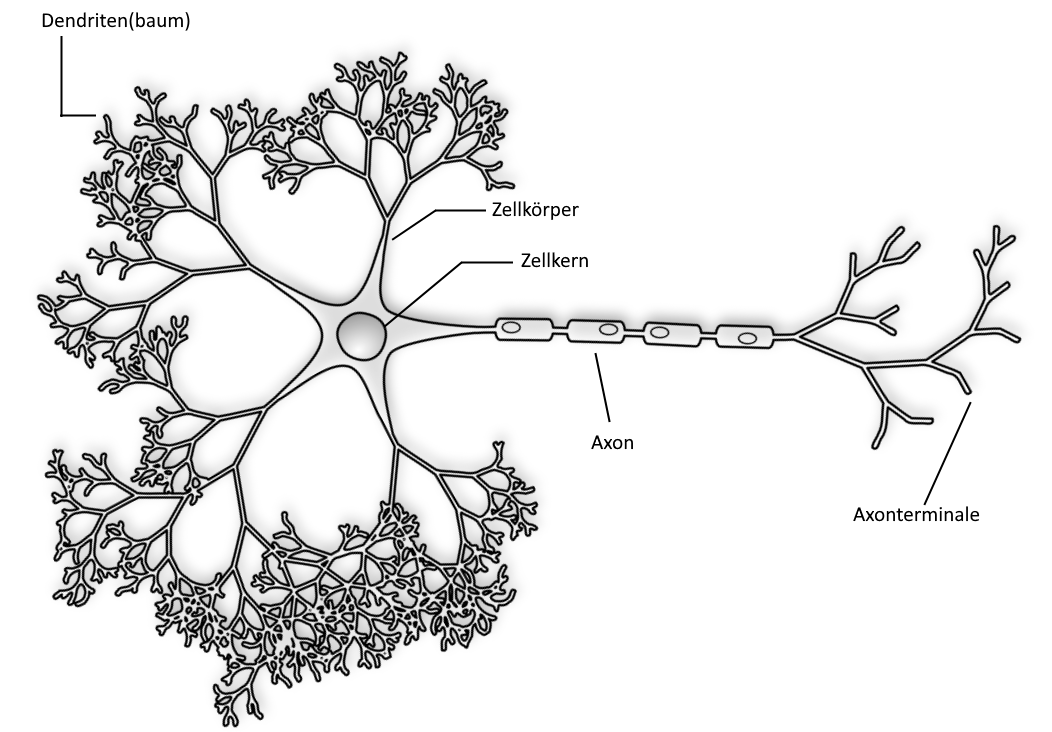
\includegraphics[scale=0.35]{Abbildungen/biologischesNeuron.png}
 \caption{Das menschliche Neuron}
 \label{fig:biologisches_neuron}
\end{figure}


Jedes Neuron hat dabei sogenannte \textit{Dendriten}, die quasi als Eingang für die Signale und Informationen angesehen werden können. In den \textit{Dendriten} kommen chemische Signale von anderen Neuronen an, die in ganz kleine elektrische Ströme umgewandelt werden. Von dort aus gelangen diese Ströme in den inneren \textit{Zellkörper}. Dieser ist mit den \textit{Axonen} - bis zu einem Meter langen Fortsätzen der \textit{Zellkörper} - verbunden, welche an die \textit{Dendriten} anderer Neuronen münden und hier durch Neurotransmitter wie Noradrenalin, Acetylcholin, Dopamin oder Serotonin verschieden starke chemische Signale abgeben, die wieder in unterschiedliche elektrische Signale umgewandelt werden (vgl . \cite[29-30]{Steinwendner2019} \& \cite{rundfunk_2019}). Es entsteht ein riesengroßes Netzwerk aus diesen Neuronen. Grundlegend ist hier auch, dass sowohl die \textit{Dendriten}, als auch die \textit{Axone} über \textit{Synapsen} mit dem \textit{Zellkörper} verbunden sind. Diese \textit{Synapsen} sind für die Umwandlung von chemischen Signalen in elektrische verantwortlich und können das Signal hemmen oder erregen. Dadurch haben verschiedene Neurone unterschiedliche ``Wichtigkeiten'' oder auch Einflüsse.

\subsection{Das künstliche Neuron}
Um sich dem biologischen Neuron mit der mathematischen Kopie anzunähern, hilft es eine vorerst simplifizierte Darstellung zu wählen. Das folgende Modell bezieht sich nur auf den Teil des biologischen Neurons von den \textit{Dendriten} bis zu den \textit{Zellkörpern}, die dann wieder als Eingabesignal für andere \textit{Dendriten} verwendet werden (s. \cref{fig:kuenstliches_neuron} ).




\begin{figure}[h]
 \centering
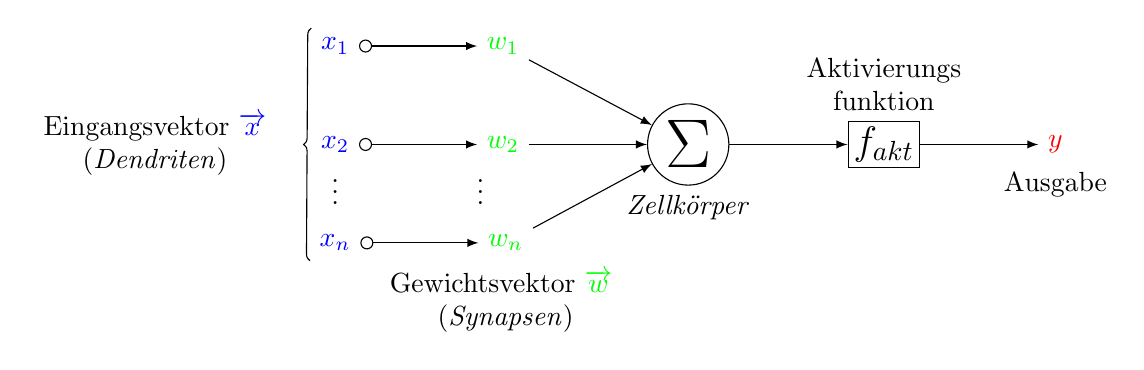
\begin{tikzpicture}[
init/.style={
  draw,
  circle,
  inner sep=2pt,
  font=\Huge,
  join = by -latex
},
squa/.style={
  draw,
  inner sep=2pt,
  font=\Large,
  join = by -latex
},
start chain=2,node distance=15mm
]
\node[on chain=2] 
  (x2) {$\color{blue}{x_2}$};
\node[on chain=2,join=by o-latex] 
  {$\color{green}{w_2}$};
\node[on chain=2,label=below:{\parbox{2cm}{\centering{ \textit{Zellkörper}}}},init] (sigma) 
  {$\displaystyle\Sigma$};
\node[on chain=2,squa,label=above:{\parbox{2cm}{\centering Aktivierungs \\ funktion}}]   
  {$f_{akt}$};
\node[on chain=2,label=below:Ausgabe,join=by -latex] 
  {$\color{red}{y}$};
\begin{scope}[start chain=1]
\node[on chain=1] at (0,1.25cm) 
  (x1) {$\color{blue}{x_1}$};
\node[on chain=1,join=by o-latex] 
  (w1) {$\color{green}{w_1}$};
\end{scope}
\begin{scope}[start chain=3]
\node[on chain=3] at (0,-0.5cm) 
  (dots1) {$\vdots$};
\node[on chain=3] 
  (dots2) {$\vdots$};
\end{scope}
\begin{scope}[start chain=4]
\node[on chain=4] at (0,-1.25cm) 
  (xn) {$\color{blue}{x_n}$};
\node[on chain=4,label=below:{\parbox{3cm}{\centering{ Gewichtsvektor \color {green} $\overrightarrow w$ \color{black} \\ (\textit{Synapsen})}}},join=by o-latex] 
  (wn) {$\color{green}{w_n}$};
\end{scope}

\draw[-latex] (w1) -- (sigma);
\draw[-latex] (wn) -- (sigma);

\draw[decorate,decoration={brace,mirror}] (x1.north west) -- node[left=10pt] {{\parbox{3cm}{\centering Eingangsvektor \color{blue}{$\overrightarrow x$} \\ \color{black}{(\textit{Dendriten})}}}} (xn.south west);
\end{tikzpicture}
\caption{Ein künstliches Neuron}
\label{fig:kuenstliches_neuron}
\end{figure}

Generell werden alle Elemente des künstlichen Neurons mithilfe der Mathematik realisiert, angefangen bei den \textit{Dendriten}, die als Eingangsvektor \color{blue}{$\overrightarrow x$} \color{black} dargestellt werden. Dieser besteht aus n Elementen, sein letzes Element ist \color{blue}{$x_n$} \color{black}. Die Synapsen finden Entsprechung in den sogenannten \textit{Gewichten}, die hier als Gewichtsvektor \color{green} $\overrightarrow w$ \color{black} angegeben sind. Das Signal, das dann im \textit{Zellkörper} ankommt, ist die \textit{gewichtete Summe} aller Produkte zwischen $\color{blue} x_i$ \color{black} und \color{green} $w_i$ \color{black}:
\begin{displaymath}
 \sum_{i=1}^{n} \color{blue} x_i \color{black} \cdot \color{green} w_i
\end{displaymath}
\color{black}

Dieser im \textit{Zellkörper} ankommende ``Reiz'' wird dann in eine \textit{Aktivierungsfunktion} weitergeleitet. Es gibt sehr viele unterschiedliche Aktivierungsfunktionen - lineare und nicht lineare - , die für eine feinere Abstufung des Ergebnisses oder eine klare Trennung zwischen 1 und 0, wahr und falsch, Hund oder Katze zu gebrauchen sind. Geläufig ist die \textit{Sigmoid-Funktion} (siehe \cref{fig:sigmoid} ), weil ihre Ausgabe zwischen 0 und 1 liegt. Das ist besonders nützlich, wenn es um eine Wahrscheinlichkeitsvorhersage geht.


\begin{figure}[h]
\begin{minipage}{.3\textwidth}
  \centering
  \begin{displaymath}
   sig(t) = \frac{1}{1 + e^{-t}}
  \end{displaymath}
\end{minipage}%
\begin{minipage}{0.6\textwidth}
  \centering
  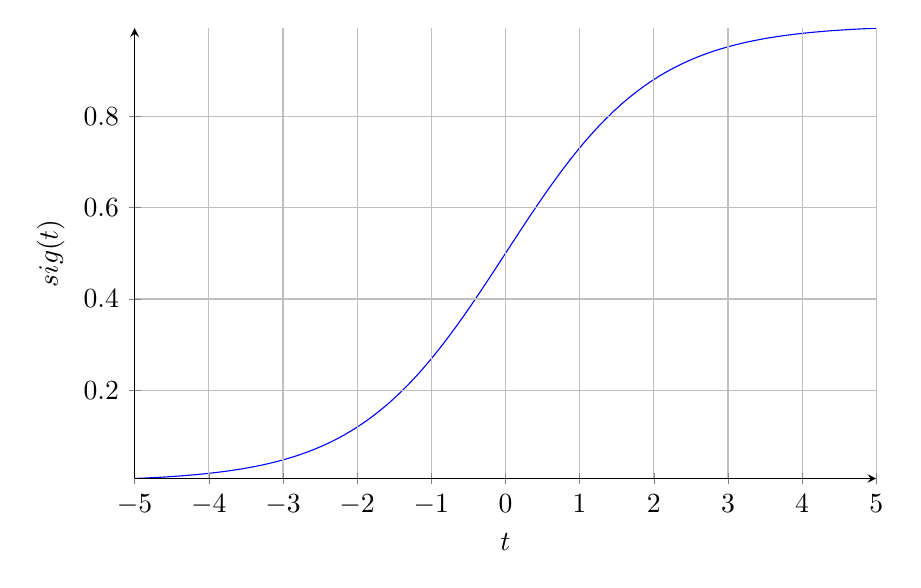
\begin{tikzpicture}
    \begin{axis}[
%         title = {Sigmoid Funktion},
        axis on top = true,
        axis x line = bottom,
        axis y line = left,
        grid = major,
        height = 7.3cm,
        width = 11cm,
        xlabel = $t$,
        ylabel = $sig(t)$
    ]
        \addplot[
            blue,
            domain = -5:5,
            samples = 100
        ]
            {1/(1+exp(-x))};
    \end{axis}
   \end{tikzpicture}
  \label{fig:sigmoid}
\end{minipage}
\caption{Sigmoid Funktion}
\label{fig:sigmoid}
\end{figure}


Diese Sigmoid-Funktion lässt sich auch implementieren. Hierbei wird die mathematische Bibliothek \textit{numpy} verwendet, da diese Operatoren oder Terme auf Listen oder Matrizen anwenden kann. Liegt zum Beispiel eine Matrix mit gewichteten Summen vor, lässt sich diese Funktion direkt auf jeden Wert in der Matrix gleichzeitig anwenden (siehe \cref{fig:sigmoid_implementation} ).

\begin{figure}[h]
\begin{lstlisting}
import numpy as np

 def sigmoid(x):
    return 1/(1+np.exp(-x))
\end{lstlisting}
\caption{Sigmoid-Funktion Implementation}
\label{fig:sigmoid_implementation}
\end{figure}


(vgl. \cite[30-32]{Steinwendner2019} )


\subsection{FeedForward-Netz}
Um komplexere Aufgaben zu lösen, wird mehr als ein einziges Neuron benötigt. Es müssen mehrere Neuronen miteinander verbunden werden, dass sie - genauso wie auch beim Menschlichen Gehirn - untereinander kommunizieren können. Es gibt hierbei viele verschiedene Arten, die Neuronen untereinander zu verbinden und sie in unterschiedlichen Schichten oder Strukturen - auch \textit{Topologien} - auszurichten. Das Verfahren \textit{Neuroevolution} braucht hauptsächlich das sogenannte \textit{Mehrschichtige FeedForward-Netz}. Es liegen mehrere nacheinander verkettete Schichten von Neuronen vor, die von links nach rechts befeuert werden (siehe \cref{fig:ffnet} ).
\begin{figure}[h]
 \centering
 

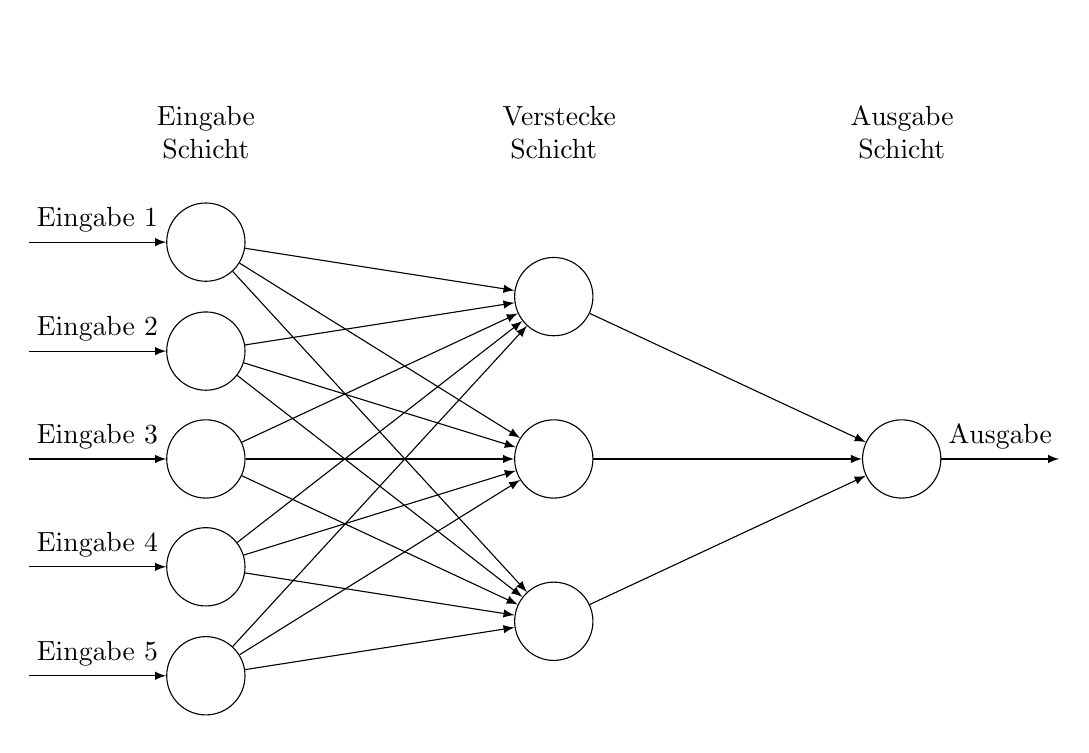
\begin{tikzpicture}[
plain/.style={
  draw=none,
  fill=none,
  },
net/.style={
  matrix of nodes,
  nodes={
    draw,
    circle,
    inner sep=10pt
    },
  nodes in empty cells,
  column sep=2cm,
  row sep=-9pt
  },
>=latex
]
\matrix[net] (mat)
{
|[plain]| \parbox{1.3cm}{\centering Eingabe\\Schicht} & |[plain]| \parbox{1.3cm}{\centering Verstecke\\Schicht} & |[plain]| \parbox{1.3cm}{\centering Ausgabe\\Schicht} \\
& |[plain]| \\
|[plain]| & \\
& |[plain]| \\
  |[plain]| & |[plain]| \\
& & \\
  |[plain]| & |[plain]| \\
& |[plain]| \\
  |[plain]| & \\
& |[plain]| \\    };
\foreach \ai [count=\mi ]in {2,4,...,10}
  \draw[<-] (mat-\ai-1) -- node[above] {Eingabe \mi} +(-2.25cm,0);
\foreach \ai in {2,4,...,10}
{\foreach \aii in {3,6,9}
  \draw[->] (mat-\ai-1) -- (mat-\aii-2);
}
\foreach \ai in {3,6,9}
  \draw[->] (mat-\ai-2) -- (mat-6-3);
\draw[->] (mat-6-3) -- node[above] {Ausgabe} +(2cm,0);
\end{tikzpicture}
\caption{Mehrschichtiges Feedforward Netz}
\label{fig:ffnet}
\end{figure}

Diese Mehrschichtigen FeedForward Netze bestehen - wie der Name verrät - aus mehreren Schichten, dessen erste als \textit{Eingabeschicht} verstanden wird. Die letzte ist logischerweise als \textit{Ausgabeschicht} zu bezeichnen. Alle Schichten dazwischen - hier können auch mehrere auftreten - werden als \textit{``versteckte Schichten''} (engl.: hidden layers) bezeichnet. Dieser Name kommt daher, dass der Benutzer, der das Netz aufsetzt, quasi keine Interakion mit diesen Schichten hat und diese so als ``Blackbox'' verstanden werden können. Um ein solches Neuronales Netz zu implementieren, reicht es, die Gewichte und die Aktivierungsfunktionen zu speichern, denn die Eingabewerte sind immer unterschiedlich (siehe \cref{fig:ffn_implementierung} ).

\begin{figure}[h]
 \lstinputlisting[firstline=16,lastline=30]{Programmcode/Fixed_Top_CartPole.py}
 \caption{Neuronales Netzwerk Implementation}
 \label{fig:ffn_implementierung}
\end{figure}

(vgl. \cite{feed-forward_nn} )
\newpage

\subsection{Propagation}

Links, am Anfang des Netzes in der Eingabeschicht, werden Eingaben getätigt. Hier werden zum Beispiel die Pixel eines Bildes eingegeben. Dann finden die oben benannten Berechnungen der \textit{gewichteten Summen} in jedem Neuron statt, die durch eine \textit{Aktivierungsfunktion} laufen und dann an das jeweilige verbundene Neuron in der ersten \textit{verstecken Schicht} weitergeleitet werden. Dieser Prozess findet solange statt, bis das \textit{Ausgabeneuron} - auch hier kann es mehrere geben - erreicht ist. Die Ausgabe findet in Form von Zahlen statt (siehe \cref{fig:propagation} ). Ob auf dem eingegebenen Bild laut dem Neuronalen Netz ein Hund oder eine Katze zu 
erkennen sein soll, wird zum Beispiel durch eine Zahl von 0 bis 1 ausgegeben. Die \textit{Ausgabeneuronen} sind für die Überlieferung oder Ausgabe der Aktion oder Entscheidung des Netzes verantwortlich. 

\begin{figure}[h]
 \lstinputlisting[firstline=32,lastline=40]{Programmcode/Fixed_Top_CartPole.py}
 \caption{Befeuerung - Propagation Implementation}
 \label{fig:propagation}
\end{figure}

(vgl. \cite{zell_2003} )

\subsection*{Lernstrategien}
Bisher wurde beschrieben, wie ein Feedforward Netz funktioniert. Analogisch zum Menschen muss aber auch jedes Neuronale Netz erst einmal etwas lernen. Unter ``Lernen'' versteht man bei künstlichen Neuronalen Netzen das Anpassen der Gewichte. Diese bleiben bei der Propagation immer gleich, unabhängig vom Eingangsvektor. Wie effizient ein Netz ist, hängt demnach nicht nur von der \textit{Topologie} ab, sondern auch von den \textit{Gewichtsvektoren}.

Bei der Arbeit mit Neuronalen Netzen und zum Beispiel der Klassifizierung zwischen Hund und Katze anhand eines Bildes, muss zunächst mit ernüchternden Ergebnissen gerechnet werden. Ohne Training trifft das Neuronale Netz nur willkürliche Entscheidungen - wie ein kleines Kind, das noch nicht weiß, was Hunde von Katzen unterscheidet. 

Um die Gewichte entsprechend immer besser anzupassen, gibt es zahlreiche Lernstrategien, die unterschiedliche Anwendungsgebiete finden. Bekannt ist die sogenannte \textit{Backpropagation}. Hierbei wird händisch eine Klassifizierung  von zum Beispiel 10.000 Hundebildern sowie 10.000 Katzenbildern erstellt. Das Netz kriegt immer ein Eingabebild, das es klassifizieren soll. Diese Vorraussagung des Netzes wird anschließend mit dem wahren Inhalt des Bildes (Hund oder Katze) verglichen und es findet eine \textit{Fehlerauswertung} mithilfe des Verfahrens \textit{Gradient descent} statt, die die Gewichte immer besser anpasst, sodass nach tausenden von Wiederholungen eine richtige Klassifizierung sehr viel wahrscheinlicher wird. Je mehr ein Neuronales Netz trainiert wird und je mehr Eingabedaten dabei verwendet werden, desto präziser ist das Ergebnis, also seine Fähigkeit, die richtige Aussage über die Eingabedaten zu treffen (vgl. \cite[149ff]{Steinwendner2019} ). 

Das Verfahren \textit{Neuroevolution} ist ebenfalls eine Lernstrategie, basiert aber im Gegensatz zu der Backpropagation auf naturähnlicher Evolution der Neuronalen Netzwerke. 

\section{Neuroevolution}
\label{sec:neuroevolution}
Im Gegensatz zum \textit{Backpropagation}-Verfahren benötigt die Neuroevolution nicht unbedingt unzählige korrekte ``Lerndaten''. Soll der  Algorithmus zum Beispiel das Spielen eines Spiels lernen, reicht es nach jedem Durchgang eine Rückmeldung (engl.: ``fitness'') über den Erfolg mit dem aktuellen Neuronalen Netz zu erhalten. Daraufhin findet eine eventuelle Anpassung der Gewichte oder der Topologie statt (siehe \cref{fig:neuroevolution}) (vgl. \cite{stanley_2017}, \cite[25-28]{eiben_smith_2016} ).

\begin{figure}[h]
 \centering
 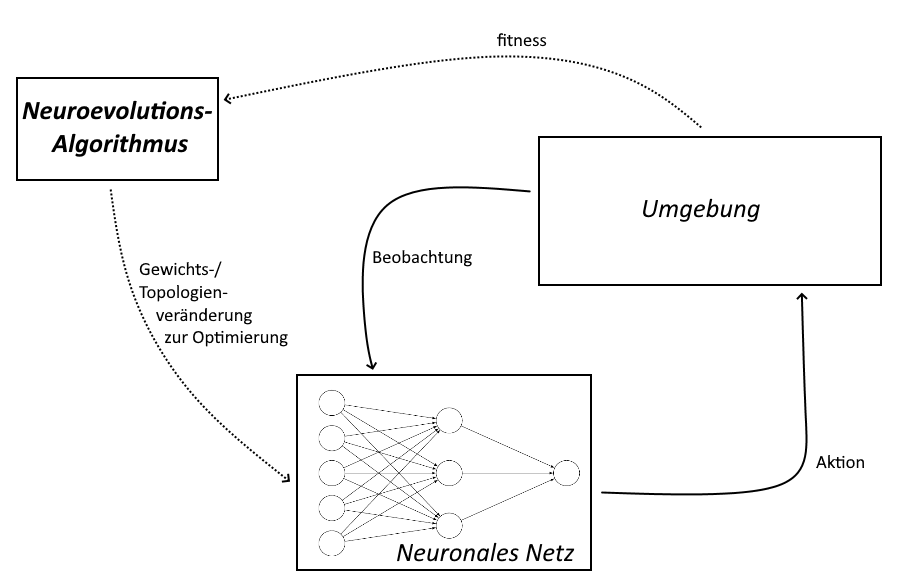
\includegraphics[scale=0.5]{Abbildungen/Neuroevolution.png}
 \caption{Neuroevolution}
 \label{fig:neuroevolution}
\end{figure}

Die Veränderung der Topologie durch das Neuroevolutionsverfahren ist erst später entstanden, hier fehlte noch das richtige System - die Topologienveränderung führt schnell zu vielen Problemen. In den nächsten Abschnitten wird die Neuroevolution deswegen zunächst mit festen Topologien (engl.: ``fixed topologies'') implementiert.

\subsection{Generationsbegriff}
Neuroevolutionsverfahren werden auch als \textit{evolutionäre Algorithmen} bezeichnet. Diese Art von Algorithmen orientiert sich an der Natur und ist generationsbasiert. Jeder Lernschritt findet in Form einer \textit{Generation} statt. Jede einzelne Generation besteht aus einer Bevölkerung von vielen einzelnen ``Agenten'', die mit verschiedenen Neuronalen Netzen unterschiedliche Lösungsansätze für das zu lösende Problem anbieten (siehe \cref{fig:agent} ). Die Neuronalen Netze und somit die Agenten der ersten Generation werden meistens per Zufall generiert (siehe \cref{fig:gen_random} ). Es wird nicht mehr nur ein Neuronales Netz wie bei der \textit{Backpropagation} verwendet, sondern mehrere - manchmal bis zu tausend Stück - danach wird ausgewählt, welches Netz am besten abgeschnitten hat (vgl. \cite[25-28]{eiben_smith_2016} ). \\

\begin{figure}[h]
 \lstinputlisting[firstline=43,lastline=47]{Programmcode/Fixed_Top_CartPole.py}
 \caption{Agent Implementation}
 \label{fig:agent}
\end{figure}

\begin{figure}[h]
 \lstinputlisting[firstline=51,lastline=52]{Programmcode/Fixed_Top_CartPole.py}
 \caption{Zufällige Generationserzeugung Implementation}
 \label{fig:gen_random}
\end{figure}

\subsection{Fitness-function}
Die einzelnen Agenten interagieren während einer Generation auf ihre Art und Weise mit der Umgebung, solange bis die Umgebung eine Rückmeldung - zum Beispiel über den Erfolg in einer bestimmten Situation - liefert. Dafür wird die sogenannte \textit{``Fitness function''} genutzt, welche von der Umgebung realisiert wird und von Problem zu Problem unterschiedlich ist. Mithilfe einer Zahl wird hier jedem Agenten eine Information gegeben, wie gut er mit seiner Strategie - seinem Neuronalen Netz - abgeschnitten hat. Je höher die Zahl ist, desto besser war die Strategie (vgl. \cite[30]{eiben_smith_2016} ).


\subsection{Selection}
Um die einzelnen Agenten zu verbessern und besser auf den nächsten Durchgang der Umgebung vorzubereiten, wird direkt die nächste Generation erstellt. Zur bestmöglichen Anpassung der Agenten werden daher zunächst diejenigen herausgesucht, die in der vorherigen Generation am besten abgeschnitten haben - sprich diejenigen, die die höchsten \textit{fitness}-Werte hatten. Dieser Prozess nennt sich \textit{Selection}, wie nach Charles Darwin überleben die Anpassungsfähigsten oder zumindest die, die besser abschneiden, als die anderen. \\
Zur Auswahl der besten Lösungen gibt es viele Ansätze. Bei meiner Implementation werden alle Agenten der gesamten Generation zuerst sortiert. Danach werden die besten 50\% zum ``Überleben'' ausgewählt, der Rest wird verworfen (siehe \cref{fig:selection} ) (vgl. \cite[31 - 33]{eiben_smith_2016} ).

\begin{figure}[h]
 \lstinputlisting[firstline=54,lastline=57]{Programmcode/Fixed_Top_CartPole.py}
 \caption{Selection Implementation}
 \label{fig:selection}
\end{figure}


\subsection{Crossover}
\label{subsec:crossover}
Der nächste Schritt der Reproduktion der alten und somit Erzeugung der neuen Generation nennt sich ``Crossover'' - zu Deutsch ``Kreuzung''. Für den nächsten Durchgang wird wieder eine gesamte Population benötigt, die es erst zu erstellen gilt. Für das Crossover gibt es ebenfalls viele unterschiedliche Verfahren und Vorgehensweisen. In meiner Implementation wird zunächst der Gewinner mit dem höchsten Fitness-Wert der letzen Generation ohne Änderungen übernommen, danach wird Agent um Agent aufgefüllt, bis die Populationsgröße wieder erreicht ist. 

Bei jedem Agenten, der in diesem Prozess hinzugefügt wird, wird zwischen Klonen und Kreuzen unterschieden. Zu einer 25\%-igen Wahrscheinlichkeit wird ein Agent aus der alten Generation ohne Kreuzvorgang übernommen. Trifft hingegen die andere, 75\%-ige Wahrscheinlichkeit ein, werden - wie vorher beschrieben - zwei Eltern aus der vorherigen Generation gesucht und gekreuzt, indem die Gewichte der beiden gemischt werden. Für diese Kreuzung zweier Gene in Form von Gewichten wird ein Punkt per Zufall ausgesucht, an dem die Gewichte des ersten und des zweiten Elternteils geteilt werden. Das Kind bekommt dann einen Teil des Gewichtsvektors vom ersten Elternteil und den anderen Teil vom anderen Elternteil, sodass wieder ein vollständiger, gekreuzter Gewichtsvektor entsteht (siehe \cref{fig:crossover_bild} ). 


\begin{figure}[h]
\centering
 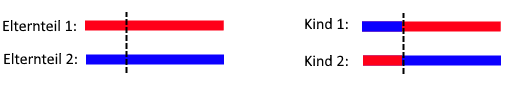
\includegraphics[scale=0.75]{Abbildungen/Crossover.png}
 \caption{Crossover - Kreuzung zweier Neuronale Netze}
 \label{fig:crossover_bild}
\end{figure}


Unabhängig davon, ob nur geklont oder auch gekreuzt wurde, wird dann bei jedem neu entstandenen Kind zu einer festgelegten Wahrscheinlichkeit eine Mutation durchgeführt (siehe  \cref{subsec:mutation} ).

Problematisch erscheint es, dass die Gewichte nicht als eine simple lineare Liste vorliegen, sondern teilweise auch als komplexe Matrix. Damit diese gekreuzt werden können, müssen sie erst in eine lineare Liste konvertiert werden (siehe \cref{fig:matrix} ). Bevor das geschieht, werden die Größen der Dimension in einer Variable festgehalten, um diese Dimension später wiederherstellen zu können. Danach wird unter anderem die Funktion \lstinline|flatten()| der Bibliothek \textit{numpy} verwendet, die einen mehrdimensionalen Array in eine einzige Dimension herunterbrechen kann. Nun kann diese lineare Liste an einem zufälligen Index gespalten werden und nur einen Teil für den Nachwuchs zur Verfügung stellen. 

Das entstandene Kind hat nun Gene sowohl vom einen als auch vom anderen Elternteil. Um die oben beschriebene Zurückführung in die eigentliche Dimension zu erledigen, wird die Funktion \lstinline|unflatten()| definiert. Sie nimmt den rohen linearen Array und den strukturellen Aufbau entgegen und gibt die zurückgeführte Matrix zurück (siehe \cref{fig:unflatten} ). 

\begin{figure}[h]
 \lstinputlisting[firstline=59,lastline=66]{Programmcode/Fixed_Top_CartPole.py}
 \caption{Unflatten-Funktion Implementation}
 \label{fig:unflatten}
\end{figure}
\newpage

Das neu erzeugte Kind wird als neuer Agent in die Population eingepflegt. Ist die Population voll, dann ist der Crossovervorgang abgeschlossen (vgl. \cite[31 - 33]{eiben_smith_2016} ).

Rückwirkend sollte noch einmal auf die Auswahl der Elternpaare eingegangen werden. Diese werden nicht nur zufällig aus der Menge der ``überlebenden Hälfte'' ausgewählt, sondern nach der Exponentialverteilung gewählt. Hier haben in der vorherigen Generation besser Abschneidende eine höhere Wahrscheinlichkeit ausgewählt zu werden, als schlechter Abschneidende. Die aus dem Crossover hervorgehenden Agenten sind daher potentiell eher von den besseren Agenten der vorherigen Generation abhängig. Die Exponentialverteilung kann durch viele Methoden implementiert werden. Für die Generierung von exponentiell abnehmenden Zufallszahlen wie in diesem Beispiel verwendet man dabei unter anderem die \textit{Wahrscheinlichkeitsdichtefunktion}. Diese ist definiert als:


\begin{equation}
    f(x;\lambda) = \begin{cases}
    \lambda  e^{-(\lambda x)} & x \ge 0, \\
    0 & x < 0.
 \end{cases}
\end{equation}
Dabei ist $\lambda$ ein Parameter für die Verteilung. Damit für jede beliebige Populationsgröße immer eine gleichmäßig leicht nach links geneigte Wahrscheinlichkeitsdichte auftritt, - sei \textit{n} definiert als Populationsgröße - wird lambda mit 
\begin{equation}
    \lambda = n^{-1} = \frac{1}{n}
\end{equation}
von der Populationsgröße abhängig gemacht. Diese Wahrscheinlichkeitsdichtefunktion wird dann auf jeden Index eines möglichen Elternteils angewandt, sodass sich ein Array mit unterschiedlichen Wahrscheinlichkeiten zur Auswahl ergibt, in dem die weiter links orientierten Indexe, welche den besseren Agenten der letzten Generation entsprechen, eine höhere Wahrscheinlichkeit haben, für den Crossover gewählt zu werden. Implementiert wird diese Wahrscheinlichkeitsdichtefunktion mithilfe der Bibliothek \textit{scipy.stats} und der Funktion \lstinline|expon.pdf(x, scale)|, die mit \textit{x} den Populationsarry mit Indexen und mit \textit{scale} ein invertiertes lambda, $\frac{1}{\lambda}$ entgegennimmt. 
Anschließend wird eine gleichmäßig verteilte Zufallszahl erzeugt und mit der Gesamtsumme der Wahrscheinlichkeitsdichtefunktion multipliziert. Der zurückzugebene und ausgewählte Index ist der, der links vom Start des Arrays aus im Bereich dieser Zufallszahl liegt (siehe \cref{fig:get_skewed_random} ). (vgl. \cite{wikipedia_2021_exp_dist}, \cite{scipy_stats_expon})

\begin{figure}[h]
 \lstinputlisting[firstline=68,lastline=77]{Programmcode/Fixed_Top_CartPole.py}
 \caption{Zufall per Exponentialverteilung Implementation}
 \label{fig:get_skewed_random}
\end{figure}


Zusammengefasst sieht die Crossover Funktion wie folgt aus (siehe \cref{fig:crossover} ).

\begin{figure}[h]
 \lstinputlisting[firstline=79,lastline=97]{Programmcode/Fixed_Top_CartPole.py}
 \caption{Crossover-Funktion Implementation}
 \label{fig:crossover}
\end{figure}



\subsection{Mutation}
\label{subsec:mutation}
Wie bereits in \cref{subsec:crossover} angerissen wurde, wird für jedes neue Kind und jeden neu erzeugten Agenten eine \textit{Mutation} durchgeführt. Diese hat den Sinn neue Variation und Innovation einzubringen. Zu einer bestimmten Wahrscheinlichkeit, die sich in dieser Implementation auf 10\% beläuft, wird ein zufälliges Gewicht durch einen ebenfalls per Zufall erzeugten Wert ersetzt. Dabei wird dieselbe Technik der Konvertierung und Zurückführung in eine lineare Liste benutzt, wie bereits oben beschrieben (siehe \cref{fig:mutation} ). Die Größe der Wahrscheinlichkeit muss dabei vorsichtig gewählt werden. Wenn sie zu groß ist, wird ein zu unbeständiger, fast zufälliger Verlauf erscheinen. Wählt man die Wahrscheinlichkeit zu niedrig, entwickelt sich das System zu langsam, da keine Innovation vorhanden ist, auf der eine neue Vorgehensweise oder Strategie basieren könnte, die zur Lösung des Problems beiträgt. Außerdem assimilieren sich die unterschiedlichen Agenten bei einer zu geringen Mutationsrate viel schneller, sodass der Lernprozess noch länger dauert (vgl. \cite[31 - 32]{eiben_smith_2016} ).

\begin{figure}[h]
 \lstinputlisting[firstline=99,lastline=113]{Programmcode/Fixed_Top_CartPole.py}
 \caption{Mutation-Funktion Implementation}
 \label{fig:mutation}
\end{figure}



\section{Testen der Implementation und Fazit}

\subsection{Der Lernprozess am Beispiel der ``Auto-Stab'' Umgebung}
\label{sec:test}
Um den Implementierten Algorithmus zu testen, wird eine Umgebung benötigt. Das Unternehmen OpenAI aus den USA hat zum Testen von Lernverfahren und besonders zum Testen von reinforcement-learning Verfahren wie Neuroevolution das open source Projekt \textit{gym} gestartet. Dieses umfasst mehrere Beispielumgebungen, die für das Testen der Lernverfahren optimiert sind. Um den wie oben beschrieben implementierten Neuroevolutionsalgorithmus zu testen, wird die Umgebung ``CartPole-v1'' verwendet. Diese enthält einen Wagen, der sich nach links oder nach rechts bewegen kann. Das Neuronale Netz als Agent muss vor jedem Frame und zu renderndem Bild eine Entscheidung treffen: nach links fahren (0) oder nach rechts fahren (1). Es reicht daher ein einziges Ausgabeneuron. Zentral auf dem Wagen befindet sich ein Stab, den es mithilfe des Fahrverhaltens auszubalancieren gilt (siehe \cref{fig:cartpole} ). 

\begin{figure}
 \centering
 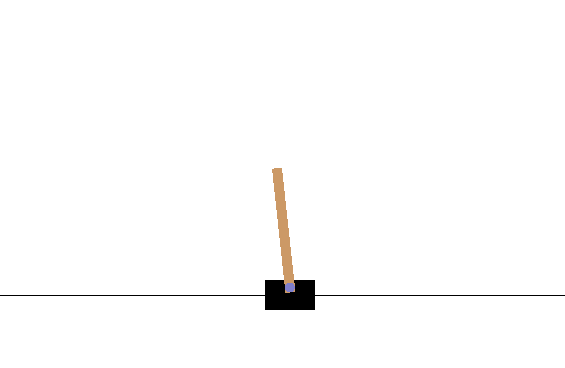
\includegraphics[scale = 0.5]{Abbildungen/cartpole.png}
 \caption{CartPole}
 \label{fig:cartpole}
\end{figure}

Der Ablauf ist genau wie zu Anfang des Abschnittes \cref{sec:neuroevolution} beschrieben. Alle Agenten der aktuellen Generation entscheiden mithilfe von verschiedenen Beobachtungen ob links oder rechts zu lenken ist. Als Beobachtung wird bei dieser Umgebung von \textit{gym} nach jedem Frame ein Array mit vier Elementen zurückgegeben. In diesem Array befinden sich die Aktuelle x-Position des Wagens (von -2.4 bis 2.4), die Geschwindigkeit des Wagens (von -$\infty$ bis +$\infty$), der Winkel des Stabes (von -41.8° bis 41.8°) und die Geschwindigkeit der Stabspitze (von -$\infty$ bis +$\infty$). Daher benötigen die Neuronalen Netze der Agenten eine Eingabeschicht mit vier Neuronen. 

Damit das Netz das Problem gut lernen kann, werden hier 5 Neuronen in der versteckten Schicht eingesetzt. Werden an dieser Stelle zu wenige Neuronen gewählt, kann das Neuronale Netz das Problem nicht richtig erlernen, da es nicht genug Fälle unterscheiden kann. Werden hingegen zu viele Neuronen verwendet, benötigt der Prozess zu viel Rechenleistung und funktioniert nur sehr langsam. 

Die Topologie des Netzes ist jedoch nicht die einzige Konstante, die es anzupassen gilt. Die Anzahl der Generationen und die Größe der Population müssen ebenfalls geregelt werden. Damit die Vorteile des Neuroevolutionsverfahrens zur Geltung kommen, sollte die Anzahl der Generationen hoch genug sein. Meistens kommt es aber vor, dass die Agenten schon eine gute Strategie herausgefunden haben, bevor die beschlossene Anzahl an Generationen durchlebt wurde. Es wird oft ein sogenannter Fitness-Threshold eingeführt. Dieser ist quasi eine Obergrenze, die zum Abbruch des Programms führt. Die Agenten haben, jetzt ausreichend gelernt, um das Problem angemessen zu meistern. Das Limit an Generationen beträgt bei meiner Implementation 200, die Populationsgröße jeweils 30 und der Fitness-Threshold wird auf 400 gesetzt.

Da bei der Auto-Stab Simulation nur eine Simulation gleichzeitig stattfinden kann, werden alle Agenten einer Generation nacheinander ausgeführt. Für jeden Zeitschritt, den der Agent überlebt, wird seine Fitness erhöht. Kippt der Stab zu weit nach links oder rechts oder bewegt sich der Wagen außerhalb des dargestellten Bildschirms, wird die aktuelle Simulation abgeschlossen und es wird mit der nächsten fortgefahren. Danach finden die oben beschriebenen Vorgange Fitness-Evaluierung, Selection, Crossover und Mutation statt. Die neu erzeugte Generation wird dann wieder Agent für Agent ausprobiert. Nach jeder Generation wird in der Konsole ein kleiner Zwischenstand ausgegeben, der Informationen über den Verlauf des Lernen abgeben soll (siehe \cref{fig:main}, eine größere Abbildung ist im Anhang zu finden). 

\begin{figure}[h]
 \lstinputlisting[firstline=117,lastline=164,basicstyle=\tiny]{Programmcode/Fixed_Top_CartPole.py}
 \caption{Ausführung des Algorithmus (kleine Darstellung)}
 \label{fig:main}
\end{figure}

Es kommt bei dieser Neuroevolutionsmethode auch dazu, dass die am Anfang zufällig gewählten Gewichte   keine gute Vorraussetzung sind, das Problem zu lösen. Die Agenten machen selbst durch die Evolution keinen Fortschritt und werden nicht besser. Das Crossover-Prinzip greift deswegen auch nicht mehr vernünftig. In diesem Fall ist durch die Zwischenstände in der Konsole zu sehen, dass die durchschnittliche Fitness sich nicht verbessert und das Programm neu gestartet werden muss. Dieser Fall tritt bei guter Werteoptimierung nur selten ein, sollte aber bei einer möglichen Fehleranalyse der Implementation berücksichtigt werden.


\label{sec:testing}

\subsection{Testen und Evaluierung des Algorithmus}
Ein großer Teil der Entwicklung eines Algorithmus ist immer das Testen seiner Effektivität. Daher soll auch der implementierte Neuroevolutionsalgorithmus getestet werden. Dazu wird der Programmcode aus Abschnitt \cref{sec:test} genutzt. Es lässt sich erkennen, dass die durchschnittliche Fitness meistens von Generation zu Generation steigt. Der Algorithmus zeigt Wirkung (siehe \cref{fig:evaluation} ). Der Lernprozess wurde auch in einem Video festgehalten (siehe \url{https://youtu.be/Xp02PP2fgyQ} ). Um den Algorithmus noch besser testen zu können, könnten noch komplexere Probleme verwendet werden und hier der Verlauf der Fitness-Kurve analysiert werden.

\begin{figure}[h]
 \centering
 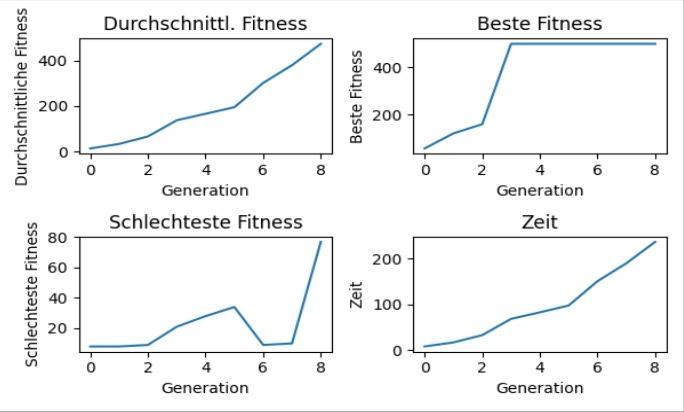
\includegraphics[scale=0.65]{Abbildungen/Evaluation.png}
 \caption{Evaluierung}
 \label{fig:evaluation}
\end{figure}

\subsection{Fazit und Ausblick}
Aus dem Ergenis dieser Implementierung der Neuroevolution mit feststehenden Topologien kann gezogen werden, dass es viele verschiedene Lernmethoden gibt, die funktionieren und Wirkung zeigen. Früher wurde die Neuroevolution als unzuverlässig empfunden, über die letzen Jahre wurde sich jedoch mehr dieser Art von reinforcement learning gewidmet, da auch die Computer immer besser wurden und mehr Rechenleistung zur Verfügung stellen. Es kommt daher auch zu vielen Neuigkeiten und neuen Verfahren auf diesem Gebiet. 2002 wurde das Verfahren NEAT veröffentlicht. Bisher gab es viele Verfahren von Neuroevolution mit feststehenden Topologien, so wie auch in der obigen Implementation. Dieses Neue Verfahren NEAT führt alternierende Topologien ein. Dabei tauchen wieder verschiedene Probleme auf, die es zu lösen gilt. 

Aus dem Überblick über die Neuroevolutions-Verfahren lässt sich erkennen, dass es in diesem Bereich so gut wie kein Falsch und kein Richtig gibt. Der einzige zu optimierende Faktor ist in dieser Gebiet - sowie in der Informatik oft - die Effizienz. 








% Literaturverzeichnis
\printbibliography[title=Literaturverzeichnis]


%Abbildungsverzeichnis
\listoffigures


\section*{Erklärung}
Hiermit versichere ich, dass ich die Arbeit selbstständig angefertigt, keine anderen als die angegebenen Hilfsmittel benutzt und die Stellen der Facharbeit, die dem Wortlaut oder im wesentlichen Inhalt aus anderen Werken entnommen wurden, mit genauer Quellenangabe kenntlich gemacht habe.

\vspace{1cm}
Ort, Datum: \underline{\hspace{12cm}}

\vspace{1cm}
Unterschrift:\underline{\hspace{12cm}}


\appendix
\newpage
\section{Abbildungen}
\subsection{Beispielmatrix mit zufälligen Gewichten}

\begin{figure}[h]
\begin{mdframed}[linecolor=black!50]
In dieser Abbildung ist der beispielhafte Gewichtsvektor eines Neuronalen Netzes mit 4 Eingangsneuronen, 5 versteckten Neuronen und 1 Ausgangsneuron dargestellt.
\begin{center}
\begin{displaymath}
\begin{bmatrix}
    -0.7255 & 0.4228 & -0.7799 & -1.2115 & -0.9617\\
    -0.3162 & 1.4284 & -0.0100 & 0.6101 & 0.5824\\
    -1.8437 & -0.3541 & -1.8160 & -0.449 & 0.1436\\
     0.0789 & 0.7453 & 0.1674 & 0.2487 & -0.903
\end{bmatrix}
\begin{bmatrix}
    -1.5728\\
    -2.3026\\
    -1.2218\\
     0.4414\\
     0.2672
\end{bmatrix}\newline
\end{displaymath}
\end{center}
Seine Struktur wird in einer Liste gespeichert als [(4, 5), (5, 1)]. Dann wird der Array auf eine Dimension heruntergebrochen:
\begin{center}
\begin{displaymath}
\begin{gathered}
[-0.7255, 0.4228, -0.7799, -1.2115, -0.9617, -0.3162, 1.4284, -0.0100, 0.6101, 0.5824,\\ 
-1.8437, -0.3541, -1.8160, -0.449, 0.1436, 0.0789, 0.7453, 0.1674, 0.2487, -0.9037,\\
-1.5728, -2.3026, -1.2218, 0.4414, 0.2672]
\end{gathered}
\end{displaymath}
\end{center}
Jetzt kann die Kreuzung starten und das enstandene Kind wieder in die ursprüngliche Form zurückgeführt werden.

 \caption{Beispielmatrix mit zufälligen Gewichten}
 \label{fig:matrix}
\end{mdframed}
\end{figure}

\subsection{Ausführung des Algorithmus (große Darstellung)}

\begin{figure}[h]
 \lstinputlisting[firstline=117,lastline=164]{Programmcode/Fixed_Top_CartPole.py}
 \caption{Ausführung des Algorithmus (große Darstellung)}
\end{figure}


\end{document}

